\documentclass[aspectratio=169]{beamer}

% 引入必要的宏包
\usepackage{amsmath, amssymb}
\usepackage{graphicx}
\usepackage{booktabs}
\usepackage{multirow}
\usepackage{array}
\usepackage{makecell}
\usepackage{xcolor}
\usepackage{tikz}
\usepackage{circuitikz} % 必须引入此宏包以支持 to[R] 语法

% 标题页信息
\title{EE P 538 \\ Additional Guidance for Phase 2}
\author{Instructor: Mahmood Hameed}
\date{Winter 2024}
\institute{Electrical Engineering \\ University of Washington}

\begin{document}

% Slide 1: Title
\begin{frame}
    \titlepage
\end{frame}

% Slide 2: Overview
\begin{frame}{Overview}
    \begin{itemize}
        \item Filter Design in Phase 2:
        \begin{itemize}
            \item Determine filter requirements given (a) Phase 2 S/N (75dB) requirement, (b) Phase 1 spectral noise output, and (c) Phase 2 passband requirement
            \item In your design, remember to EXCEED the min. or max. requirements because components inevitably degrade performance
        \end{itemize}
        \vspace{0.3cm}
        \item Noise Simulations:
        \begin{itemize}
            \item Use LT Spice for simulating spectral noise density ($V/\sqrt{Hz}$) and total (integrated) noise ($V\ rms$) for frequencies of 0.1Hz to 100MHz.
            \item Phase 2 deliverables specify ADC, which LT Spice can not simulate. Thus, Phase 2 instructions included Python code to simulate S/N at ADC output over a smaller frequency range (than LT spice)
        \end{itemize}
    \end{itemize}
\end{frame}

% Slide 3: Filter Design (1 of 3)
\begin{frame}{Filter Design (1 of 3)}
    \begin{itemize}
        \item The max. noise output from the filter ($V_{FiltOut-rms}$ in volts) from Phase 2 S/N:
        $$ V_{FiltOutMax-rms} = \frac{V_{signal-rms}}{10^{SNR/20}} = \frac{2V / (2\sqrt{2})}{10^{75/20}} $$
        \vspace{0.2cm}
        \item From Phase 1, most students have a design with referred-to-input spectral noise density of $\sim 10nV/\sqrt{Hz}$ or lower. With the voltage gain from Phase 1 of $G_v = 100$, the spectral noise density at the \underline{output} of Phase 1 is:
        $$ v_{ph1output-rms} \cong 1\mu V/\sqrt{Hz} $$
        \vspace{0.2cm}
        \item Compute the \textit{maximum} acceptable equivalent noise bandwidth of your filter:
        $$ f_{enb-max} = \left[ \frac{V_{FiltOutMax-rms}}{v_{ph1output-rms}} \right]^2 $$
    \end{itemize}
\end{frame}

% Slide 4: Filter Design (2 of 3)
\begin{frame}{Filter Design (2 of 3)}
    \begin{columns}
        \begin{column}{0.65\textwidth}
            \resizebox{\textwidth}{!}{
            \renewcommand{\arraystretch}{1.2}
            \begin{tabular}{|cc|c|ccccc|cc|}
                \hline
                \multicolumn{2}{|c|}{\cellcolor{blue!80}\textcolor{white}{\textbf{Butterworth}}} & \multicolumn{6}{c|}{\cellcolor{blue!80}\textcolor{white}{\textbf{Chebyshev}}} & \multicolumn{2}{c|}{\cellcolor{blue!80}\textcolor{white}{\textbf{Bessel}}} \\
                \multicolumn{2}{|c|}{\cellcolor{blue!80}\textcolor{white}{\textbf{(fco = 3 dB)}}} & \multicolumn{6}{c|}{\cellcolor{blue!80}\textcolor{white}{\textbf{(fco = ripple)}}} & \multicolumn{2}{c|}{\cellcolor{blue!80}\textcolor{white}{\textbf{(fco = 3 dB)}}} \\
                \hline
                \cellcolor{blue!80}\textcolor{white}{\textbf{Order}} & \cellcolor{blue!80}\textcolor{white}{\textbf{EqNBW}} & \cellcolor{blue!80}\textcolor{white}{\makecell{\textbf{Ripple} \\ \textbf{Order}}} & \cellcolor{blue!80}\textcolor{white}{\textbf{0.01 dB}} & \cellcolor{blue!80}\textcolor{white}{\textbf{0.1 dB}} & \cellcolor{blue!80}\textcolor{white}{\textbf{0.25 dB}} & \cellcolor{blue!80}\textcolor{white}{\textbf{0.5 dB}} & \cellcolor{blue!80}\textcolor{white}{\textbf{1.0 dB}} & \cellcolor{blue!80}\textcolor{white}{\textbf{Order}} & \cellcolor{blue!80}\textcolor{white}{\textbf{EqNBW}} \\
                \hline
                1 & 1.5708 & 1 &  &  &  &  &  & 1 & 1.57 \\
                2 & 1.1107 & 2 & 3.6672 & 2.1444 & 1.7449 & 1.4889 & 1.2532 & 2 & 1.56 \\
                3 & 1.0472 & 3 & 1.9642 & 1.4418 & 1.2825 & 1.1666 & 1.0411 & 3 & 1.08 \\
                4 & 1.0262 & 4 & 1.5039 & 1.2326 & 1.1405 & 1.0656 & 0.9735 & 4 & 1.04 \\
                5 & 1.0166 & 5 & 1.3114 & 1.1417 & 1.0780 & 1.0208 & 0.9433 & 5 & 1.04 \\
                6 & 1.0115 & 6 & 1.2120 & 1.0937 & 1.0448 & 0.9970 & 0.9272 & 6 & 1.04 \\
                7 & 1.0084 & 7 & 1.1537 & 1.0653 & 1.0251 & 0.9828 & 0.9175 & & \\
                8 & 1.0065 & 8 & 1.1166 & 1.0471 & 1.0125 & 0.9736 & 0.91133 & & \\
                9 & 1.0051 & 9 & 1.0914 & 1.0347 & 1.0038 & 0.9674 & 0.9071 & & \\
                10 & 1.0041 & 10 & 1.0736 & 1.0258 & 0.9977 & 0.9629 & 0.9041 & & \\
                \hline
            \end{tabular}
            }
        \end{column}
        \begin{column}{0.35\textwidth}
            \colorbox{black!70}{
            \begin{minipage}{\textwidth}
            \textcolor{white}{
            \begin{itemize}
                \item With maximum effective noise bandwidth ($f_{enb-max}$) and passband requirement ($0.5dB$ at $10KHz$), select the filter type (Bessel, Chebyshev, Butterworth) and the filter order (1,2,4, etc) from a chart or online calculator design tool
                \item Typically, design tools use a normalize frequency equal to the effective noise bandwidth ($f_{enb}$) divided by the filter cutoff frequency ($f_{co}$). \textit{Note this chart (https://www.rfcafe.com/references/electrical/filter-eqnbw.htm) specifies the attenuation (e.g. 3dB or 0.5dB) at the cutoff frequency.}
            \end{itemize}
            }
            \end{minipage}
            }
        \end{column}
    \end{columns}
\end{frame}

% Slide 5: Filter Design (3 of 3)
\begin{frame}{Filter Design (3 of 3)}
    \begin{itemize}
        \item In some of your Phase 1 designs, the spectral noise density increases at much higher (e.g. 10MHz) frequencies
        \item After first-pass implementation of your filter in Phase 2 in LT Spice, observe the noise density again (using LT Spice) at the output of the filter at high frequencies
        \item If large noise density at high frequencies continue to exist, consider adding in-line low-pass filters using passive devices (resistor \& capacitor) at the output of your first-pass implementation.
        \item These passive filters should have a higher corner frequency (e.g. 50kHz) that will significantly attenuate the 1MHz+ frequencies and will NOT impact the passband of your first-pass filter. (And use LT Spice to check after the second pass implementation.)
    \end{itemize}
\end{frame}

% Slide 6: Noise Simulation (LT Spice only)
\begin{frame}{Noise Simulation (LT Spice only)}
    \begin{center}
        \resizebox{0.75\textwidth}{!}{
        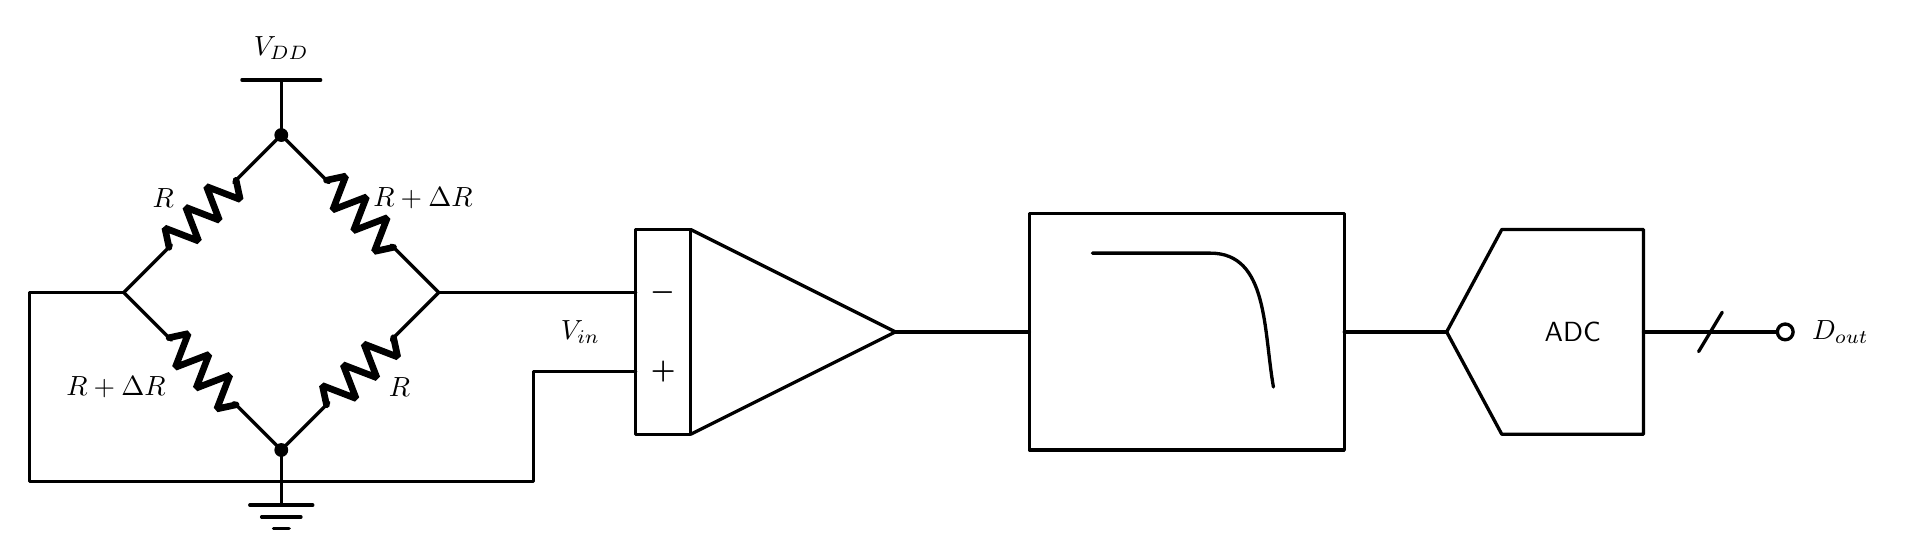
\begin{tikzpicture}[
            line width=1.2pt,
            line cap=round,
            line join=round
        ]
        % 1. Wheatstone Bridge
        \draw (-2,0) to[R] (0,2);
        \draw (0,2) to[R] (2,0);
        \draw (2,0) to[R] (0,-2);
        \draw (0,-2) to[R] (-2,0);
        \node at (-1.5, 1.2) {$R$};
        \node at (1.8, 1.2) {$R + \Delta R$};
        \node at (-2.1, -1.2) {$R + \Delta R$};
        \node at (1.5, -1.2) {$R$};
        \draw (0,2) -- (0,2.7);
        \draw (-0.5, 2.7) -- (0.5, 2.7);
        \node at (0, 3.1) {$V_{DD}$};
        \fill (0,2) circle (2.5pt); 
        \draw (0,-2) -- (0,-2.7);
        \draw (-0.4, -2.7) -- (0.4, -2.7);
        \draw (-0.25, -2.85) -- (0.25, -2.85);
        \draw (-0.1, -3.0) -- (0.1, -3.0);
        \fill (0,-2) circle (2.5pt); 

        % 2. Instrumentation Amplifier
        \draw (4.5, 0.8) rectangle (5.2, -1.8);
        \draw (5.2, 0.8) -- (7.8, -0.5) -- (5.2, -1.8);
        \node at (4.85, 0) {$\boldsymbol{-}$};
        \node at (4.85, -1) {$\boldsymbol{+}$};

        % 3. Lowpass filter
        \draw (9.5, 1) rectangle (13.5, -2);
        \draw (10.3, 0.5) -- (11.8, 0.5) to[out=0, in=100] (12.6, -1.2);

        % 4. ADC
        \draw (14.8, -0.5) -- (15.5, 0.8) -- (17.3, 0.8) -- (17.3, -1.8) -- (15.5, -1.8) -- cycle;
        \node[font=\sffamily] at (16.4, -0.5) {ADC};

        % 5. Routing
        \draw (2,0) -- (4.5,0);
        \draw (-2,0) -- (-3.2,0) -- (-3.2,-2.4) -- (3.2,-2.4) -- (3.2,-1) -- (4.5,-1);
        \node at (3.8, -0.5) {$V_{in}$};
        \draw (7.8, -0.5) -- (9.5, -0.5);
        \draw (13.5, -0.5) -- (14.8, -0.5);
        \draw (17.3, -0.5) -- (19, -0.5);
        \draw[fill=white] (19.1, -0.5) circle (0.1);
        \draw (18.0, -0.75) -- (18.3, -0.25);
        \node at (19.8, -0.5) {$D_{out}$};
        \end{tikzpicture}
        }
    \end{center}
    
    \begin{itemize}
        \item \textcolor{red}{\textbf{Phase 2 -- Filtered output before ADC}}
        \item \textit{[Note: Frequency response charts below the diagram are intentionally omitted as they require separate plotting.]}
    \end{itemize}
\end{frame}

% Slide 7: Noise Simulation (Python+Spice) 1 of 3
\begin{frame}{Noise Simulation (Python+Spice) 1 of 3}
    \begin{center}
        \resizebox{0.75\textwidth}{!}{
        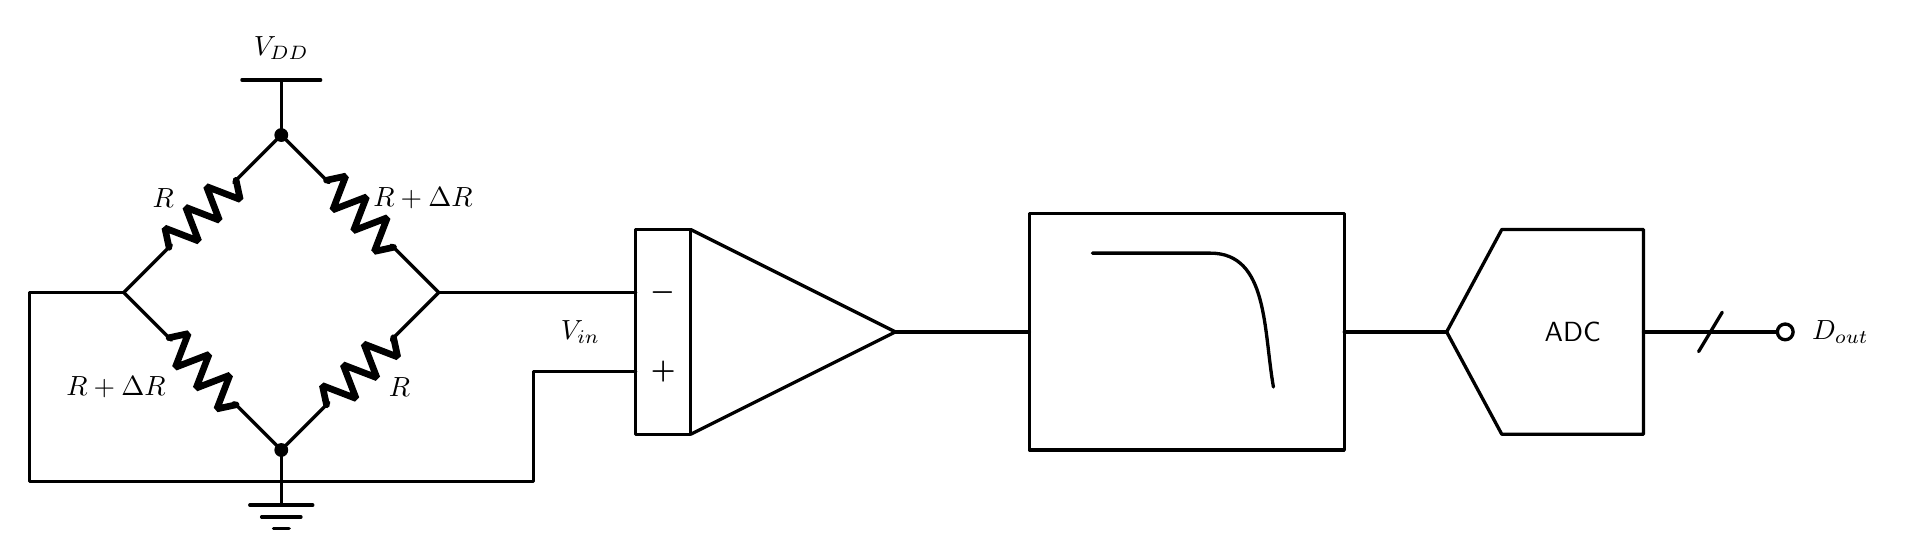
\begin{tikzpicture}[
            line width=1.2pt,
            line cap=round,
            line join=round
        ]
        % 1. Wheatstone Bridge
        \draw (-2,0) to[R] (0,2);
        \draw (0,2) to[R] (2,0);
        \draw (2,0) to[R] (0,-2);
        \draw (0,-2) to[R] (-2,0);
        \node at (-1.5, 1.2) {$R$};
        \node at (1.8, 1.2) {$R + \Delta R$};
        \node at (-2.1, -1.2) {$R + \Delta R$};
        \node at (1.5, -1.2) {$R$};
        \draw (0,2) -- (0,2.7);
        \draw (-0.5, 2.7) -- (0.5, 2.7);
        \node at (0, 3.1) {$V_{DD}$};
        \fill (0,2) circle (2.5pt); 
        \draw (0,-2) -- (0,-2.7);
        \draw (-0.4, -2.7) -- (0.4, -2.7);
        \draw (-0.25, -2.85) -- (0.25, -2.85);
        \draw (-0.1, -3.0) -- (0.1, -3.0);
        \fill (0,-2) circle (2.5pt); 

        % 2. Instrumentation Amplifier
        \draw (4.5, 0.8) rectangle (5.2, -1.8);
        \draw (5.2, 0.8) -- (7.8, -0.5) -- (5.2, -1.8);
        \node at (4.85, 0) {$\boldsymbol{-}$};
        \node at (4.85, -1) {$\boldsymbol{+}$};

        % 3. Lowpass filter
        \draw (9.5, 1) rectangle (13.5, -2);
        \draw (10.3, 0.5) -- (11.8, 0.5) to[out=0, in=100] (12.6, -1.2);

        % 4. ADC
        \draw (14.8, -0.5) -- (15.5, 0.8) -- (17.3, 0.8) -- (17.3, -1.8) -- (15.5, -1.8) -- cycle;
        \node[font=\sffamily] at (16.4, -0.5) {ADC};

        % 5. Routing
        \draw (2,0) -- (4.5,0);
        \draw (-2,0) -- (-3.2,0) -- (-3.2,-2.4) -- (3.2,-2.4) -- (3.2,-1) -- (4.5,-1);
        \node at (3.8, -0.5) {$V_{in}$};
        \draw (7.8, -0.5) -- (9.5, -0.5);
        \draw (13.5, -0.5) -- (14.8, -0.5);
        \draw (17.3, -0.5) -- (19, -0.5);
        \draw[fill=white] (19.1, -0.5) circle (0.1);
        \draw (18.0, -0.75) -- (18.3, -0.25);
        \node at (19.8, -0.5) {$D_{out}$};
        \end{tikzpicture}
        }
    \end{center}
    
    \begin{itemize}
        \item \textcolor{red}{\textbf{Spectral noise voltage density generated in Python should equal same as LT simulation}}
        \item \textcolor{red}{\textbf{Spectral noise voltage density and total (integrated) noise should exceed S/N at ADC output}}
    \end{itemize}
\end{frame}

% Slide 8: Noise Simulation (Python+Spice) 2 of 3
\begin{frame}{Noise Simulation (Python+Spice) 2 of 3}
    \begin{enumerate}
        \item Use Python to generate flat spectral noise signal from DC to 500kHz, with a spectral noise amplitude that equals the spectral noise of the Instrumentation Amplifier in the 100Hz-500kHz region. \textit{Tip: Set $vn_{rms}$ in Python equal to the integrated $\sim 100Hz-500kHz$ noise from output of Instrumentation Amplifier. (And check that spectral noise level makes sense!)}
        \vspace{0.2cm}
        \item Using output from (1) as the input to the Lowpass Filter, use LT spice to to simulate the output from the Filter. In addition, use LT spice with simulate output of the Filter given an input of a noiseless (desired) signal. \textit{Tip: use ideal voltage supplies to shift voltage up and down in LT Spice as described in next slide}
        \vspace{0.2cm}
        \item Import the two results from (2) into Python to determine the S/N after the Python code that `quantizes' and simulates an ADC
    \end{enumerate}
\end{frame}

% Slide 9: Noise Simulation (Python+Spice) 3 of 3
\begin{frame}{Noise Simulation (Python+Spice) 3 of 3}
    \begin{columns}
        \begin{column}{0.4\textwidth}
            \begin{itemize}
                \item \textit{Issue:} Output/input of Python sample uses DC average of zero volts, and WAVE format limits signals to +-1volt
                \item \textit{Solution:} Use 2.5V ideal voltage sources in Spice to shift voltage level up by 2.5V before filter and shift voltage down by 2.5V after filter
            \end{itemize}
        \end{column}
        \begin{column}{0.6\textwidth}
            % 【注意】此处为 LTSpice 软件真实截图，必须保留外部图片插入
            \begin{figure}
                \centering
                % 请确保该图片在根目录下，并取消下一行的注释
                % \includegraphics[width=\textwidth]{slide9_spice_schematic.png}
                \fbox{\parbox{\textwidth}{\centering \textit{[LTSpice Screenshot Placeholder]}}}
            \end{figure}
        \end{column}
    \end{columns}
\end{frame}

% Slide 10: Spectral and total noise voltages
\begin{frame}{Spectral and total noise voltages}
    \resizebox{\textwidth}{!}{
    \renewcommand{\arraystretch}{1.5}
    \begin{tabular}{|c|c|c|p{8.5cm}|}
        \hline
        \textbf{\makecell{Input/Output stage of \\ Top Level Design}} & \textbf{\makecell{Approximate \\ voltage noise}} & \textbf{Noise Bandwidth} & \centering\arraybackslash\textbf{Description} \\
        \hline
        \multirow{3}{*}{\parbox{4cm}{\centering \textbf{Input into Instrumentation Amp} \\ \textbf{(referred-to-input noise)}}} 
        & $\sim 10nV/\sqrt{Hz}$ & Not applicable & Approximate maximum spectral noise voltage from a few Hz to hundreds of kHz \\
        \cline{2-4}
        & $\sim 1\mu V$ & $0.1Hz - 10kHz$ & Using a perfect 10kHz filter, this integrated noise voltage will provide $\sim 77dB$ of S/N with 20mV p-to-p signal \\
        \cline{2-4}
        & $\sim 7.1\mu V$ & $0.1Hz - 500kHz$ & The equivalent noise voltage referred to input assuming 500kHz filter \\
        \hline
        \multirow{3}{*}{\parbox{4cm}{\centering \textbf{Output from Instrumentation Amp} \\ \textbf{which is Input into Filter}}} 
        & $\sim 1\mu V/\sqrt{Hz}$ & Not applicable & Because of gain, note spectral noise voltage is x100 higher than input above \\
        \cline{2-4}
        & $\sim 0.1mV$ & $0.1Hz - 10kHz$ & Noise voltage is x100 larger than input above for the same bandwidth \\
        \cline{2-4}
        & $\sim 0.7mV$ & $0.1Hz - 500kHz$ & Noise voltage is x100 larger than referred to input noise voltage above for the same 500kHz bandwidth. \textit{This is the noise voltage that should be used with Python+LT Spice (variable vn\_rms in sample Python code)} \\
        \hline
    \end{tabular}
    }
\end{frame}

\end{document}